\chapter{p4 = 2 (3 graphs)}
\newpage\begin{figure}
  \begin{tikzpicture}
      \draw
        (0.0:2) node (0){0}
        (72.0:2) node (1){1}
        (144.0:2) node (2){2}
        (216.0:2) node (3){3}
        (288.0:2) node (4){4};
      \begin{scope}[-]
        \draw (0) to (2);
        \draw (1) to (3);
        \draw (2) to (4);
        \draw (3) to (4);
      \end{scope}
    \end{tikzpicture}
\end{figure}
\begin{itemize}
\item signature: 0100010011
\item g: Graph with 5 nodes and 4 edges
\item order: 5
\item size: 4
\item max degree: 2
\item degrees: 1,1,2,2,2
\item is tree: 1
\item is bipartite: 1
\item has bridge: 1
\item is chordal: 1
\item is complete: 0
\item min cycle basis weight: 0
\item min cycle basis size: 0
\item diameter: 4
\item radius: 2
\item is eulerian: 0
\item is planar: 1
\item number of faces: 1
\item is regular: 0
\item p3: 3
\item p4: 2
\item property hash: d5f26bfbc26d2804d5819954ea369e94fa677000c68aee6b027c263c3451a1f1
\end{itemize}
\newpage
\begin{figure}
  \begin{tikzpicture}
      \draw
        (0.0:2) node (0){0}
        (72.0:2) node (1){1}
        (144.0:2) node (2){2}
        (216.0:2) node (3){3}
        (288.0:2) node (4){4};
      \begin{scope}[-]
        \draw (0) to (3);
        \draw (1) to (4);
        \draw (2) to (4);
        \draw (3) to (4);
      \end{scope}
    \end{tikzpicture}
\end{figure}
\begin{itemize}
\item signature: 0010001011
\item g: Graph with 5 nodes and 4 edges
\item order: 5
\item size: 4
\item max degree: 3
\item degrees: 1,1,1,2,3
\item is tree: 1
\item is bipartite: 1
\item has bridge: 1
\item is chordal: 1
\item is complete: 0
\item min cycle basis weight: 0
\item min cycle basis size: 0
\item diameter: 3
\item radius: 2
\item is eulerian: 0
\item is planar: 1
\item number of faces: 1
\item is regular: 0
\item p3: 4
\item p4: 2
\item property hash: e91baa75124a982a46464e7c5012b78cc4f109d5a819893139b277558f4973c4
\end{itemize}
\newpage
\begin{figure}
  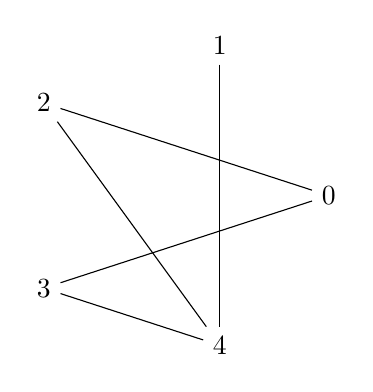
\begin{tikzpicture}
      \draw
        (0.0:2) node (0){0}
        (72.0:2) node (1){1}
        (144.0:2) node (2){2}
        (216.0:2) node (3){3}
        (288.0:2) node (4){4};
      \begin{scope}[-]
        \draw (0) to (2);
        \draw (0) to (3);
        \draw (1) to (4);
        \draw (2) to (4);
        \draw (3) to (4);
      \end{scope}
    \end{tikzpicture}
\end{figure}
\begin{itemize}
\item signature: 0110001011
\item g: Graph with 5 nodes and 5 edges
\item order: 5
\item size: 5
\item max degree: 3
\item degrees: 1,2,2,2,3
\item is tree: 0
\item is bipartite: 1
\item has bridge: 1
\item is chordal: 0
\item is complete: 0
\item min cycle basis weight: 4
\item min cycle basis size: 1
\item diameter: 3
\item radius: 2
\item is eulerian: 0
\item is planar: 1
\item number of faces: 2
\item is regular: 0
\item p3: 6
\item p4: 2
\item property hash: 02d3b8854a44375b83125826e105748a8e5daa0fee328587d5b3929392c8697c
\end{itemize}
\newpage
